%%%% Paramétrage du TD %%%%
\def\xxactivite{\ifcolle Colle 2 \else TD 4 \fi   \ifprof -- Corrigé \else \fi} % \normalsize \vspace{-.4cm}
\def\xxauteur{\textsl{Xavier Pessoles}}


\def\xxnumchapitre{Chapitre 1 \vspace{.2cm}}
\def\xxchapitre{\hspace{.12cm} Correction des systèmes}

\def\xxcompetences{%
\textsl{%
\textbf{Savoirs et compétences :}\\ \vspace{-.4cm}
\begin{itemize}[label=\ding{112},font=\color{ocre}]
\item \textit{C1-02 : }Proposer une démarche de réglage d'un correcteur.
\item \textit{C2-04 : }Mettre en œuvre une démarche de réglage d’un correcteur.
\end{itemize}
}}

\def\xxtitreexo{\noindent Machine de rééducation SysReeduc}
\def\xxsourceexo{\hspace{.2cm} \footnotesize{CCP PSI 2013}}
\def\xxauteur{\textsl{Xavier Pessoles}}

\def\xxfigures{
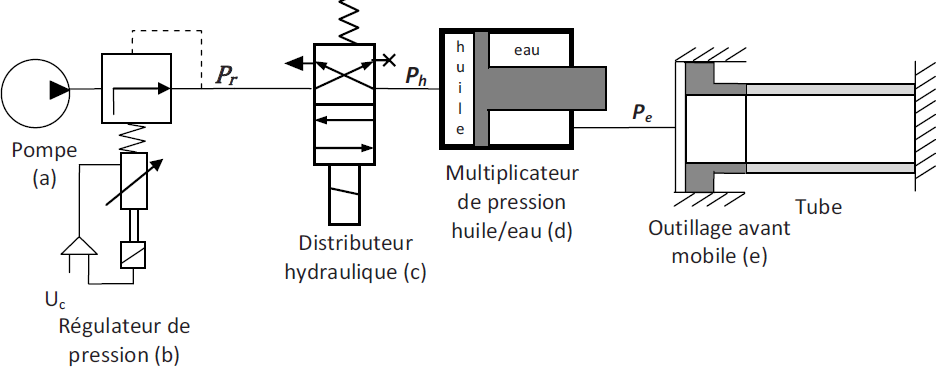
\includegraphics[width=.6\linewidth]{fig_01}
}%figues de la page de garde


\input{\repRel/Style/pagegarde_TD}
\setcounter{numques}{0}


\setlength{\columnseprule}{.1pt}

\pagestyle{fancy}
\thispagestyle{plain}

\vspace{4.7cm}

\def\columnseprulecolor{\color{ocre}}
\setlength{\columnseprule}{0.4pt} 

%%%%%%%%%%%%%%%%%%%%%%%




\setcounter{exo}{0}
\ifprof
\else
\begin{multicols}{2}
\fi
\section*{Mise en situation}

\ifprof
\else

\textit{La machine de rééducation SYS-REEDUC est issue d'un projet régional entre différents laboratoires de recherche : le CReSTIC (Centre de Recherche en Sciences et Technologies de l'Information et de la Communication) de Reims et le CRITT-MDTS (Centre Régional d'Innovation et de Transfert de Technologie) de Charleville-Mézières. L'objectif de ce projet était de réaliser un système capable d'évaluer et d'aider à la rééducation des membres inférieurs.}


\begin{center}
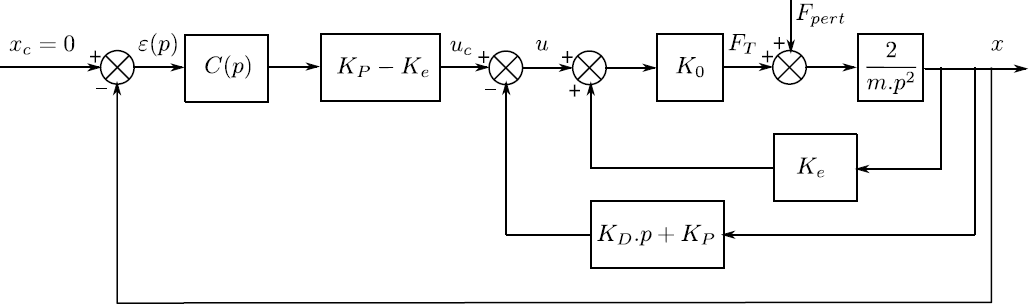
\includegraphics[width=.8\linewidth]{fig_02}
%\textit{}
\end{center}

\begin{obj}
L'objectif de cette partie est de modéliser l'asservissement du système, puis de paramétrer le correcteur pour répondre aux exigences.
\end{obj}

Pour permettre au kinésithérapeute de rééduquer les membres inférieurs du patient, on doit respecter les exigences suivantes : 
\begin{center}
\begin{tabular}{|l|c|}
\hline 
Critère & Niveau \\ \hline\hline
Angle de rotation de la cuisse &  De 0 à 150\degres \\ \hline
Effort du patient & Jusqu'à \SI{20}{N}   \\ \hline
Écart de position & Nul   \\ \hline
Marge de gain & \SI{7}{dB} mini \\ \hline
Marge de phase &  45\degres \\ \hline
Rapidité &  $t_{5\%} < \SI{0,2}{s}$ \\ \hline
Pulsation au gain unité & $\SI{50}{rad.s^{-1}}$\\
\hline
\end{tabular}
\end{center}

La structure du schéma-blocs permettant l'asservissement du déplacement longitudinal du << chariot >> (support mobile) est donnée dans la figure suivante.


\begin{center}
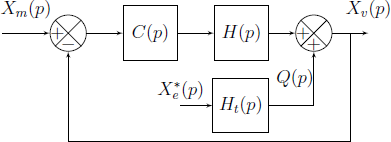
\includegraphics[width=\linewidth]{fig_03}
%\textit{}
\end{center}

\fi

\subsection*{Éléments de modélisation}

\ifprof
\else
On propose alors une modélisation par schéma-blocs dans la figure suivante. 
\begin{center}
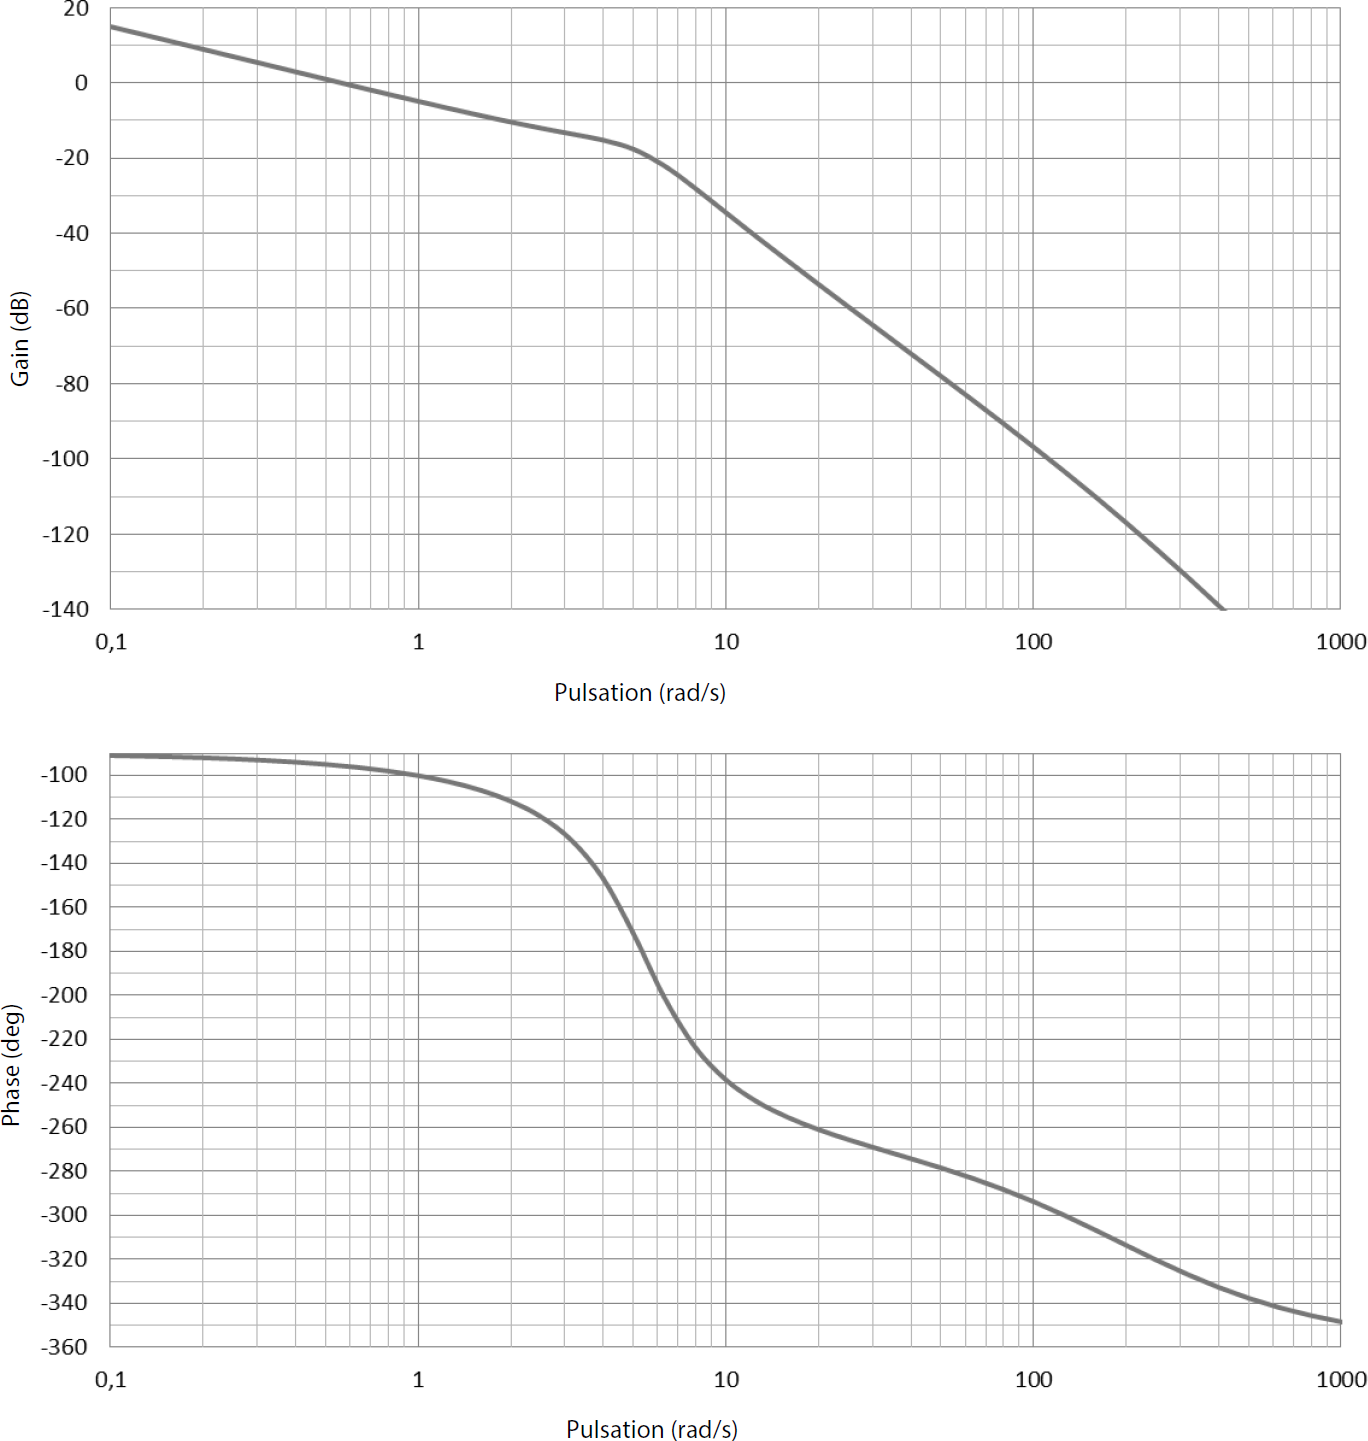
\includegraphics[width=\linewidth]{fig_04}
%\textit{}
\end{center}

Le moteur à courant continu est régi par les équations suivantes :
$ u_m(t)=e(t)+Ri(t)$, $e(t)=k_e\omega_m(t)$ et $C_{M1}(t)=k_t i(t)$. 

Une étude dynamique a mené à l'équation suivante : 
$$\left(M+m\right)r\rho_1 \dot{\omega}_m(t)=\dfrac{C_{M1}(t)}{\rho_1 r}-F_p(t)$$ avec : $M$ la masse du chariot et $m$ la masse du support de pied, $\rho_1=\dfrac{1}{10}$ le rapport de réduction du réducteur, $r=\SI{46,1}{mm}$ le rayon de la poulie du transmetteur poulie--courroie, $C_{M1}(t)$ le couple délivré par le moteur et $F_p(t)$ l'effort délivré par le patient sur le support 3. 

Le codeur incrémental possède 500 fentes équiréparties. Deux émetteurs-récepteurs positionnés en quadrature permettent de mesurer l'information. 
\fi

\question{À partir des équations proposées, déterminer les fonctions de transfert $K_1$, $K_2$, $H_3(p)$, $H_4(p)$,  $K_5$, $K_6$, $K_7$, $K_8$ et $K_9$.}
\ifprof
\begin{corrige}~\\
On a :
\begin{itemize}
\item $ u_m(t)=e(t)+Ri(t) \Rightarrow  U_m(p)=E(p)+RI(p) $ et $C_{M1}(p)=k_t I(p)$ donc $K_2 = \dfrac{k_t}{R}$;
\item $E(p)=k_e\Omega_m(p)$ et donc $K_7 = k_e$;
\item $\left(M+m\right)r\rho_1 p\Omega_m(p)=\dfrac{C_{M1}(p)}{\rho_1 r}-F_p(p) \Leftrightarrow\left(M+m\right)r^2\rho_1^2 p\Omega_m(p)=C_{M1}(p)-\rho_1 rF_p(p) $ et donc $K_9 = \rho_1 r$ et $H_3(p)=\dfrac{1}{\left(M+m\right)r^2\rho_1^2 p}$;
\item  $H_4(p)$ permet d'obtenir une position à partir d'une vitesse. Il s'agit donc d'un intégrateur et $H_4(p)=\dfrac{1}{p}$; 
\item un codeur incrémental avec 1 émetteur-récepteur permet de détecter les fentes et les << non fentes >> donc ici 1000 informations par tour. Avec un second émetteur, on double la résolution soit 2000 informations pour un tour soit $K_8  = \dfrac{2000}{2\pi}$;
\item en utilisant le réducteur et le poulie courroie, on a directement $K_5=\rho_1$ et $K_6=r$ (à convertir en mètres);
\item enfin, $K_1$ convertit des mètres en incréments. $X_c$ est la consigne que doit respectée $X$. Pour avoir un asservissement précis, il faut donc $\varepsilon = 0$ et $X=X_c$ soit $\varepsilon = 0 = K_1 X_C - K_8 \theta_m = K_1 X_C - K_8 \dfrac{X}{K_5 K_6}$. Au final, $K_1 =\dfrac{K_8}{K_5 K_6}$.
\end{itemize}
\end{corrige}
\else
\fi

\question{Montrer que le schéma-blocs peut être mis sous la forme suivante. On exprimera $A$, $B$ et $D$ en fonction des paramètres du système $r$, $\rho_1$, $k_t$, $k_e$, $R$, $M$, $m$ et $K_8$. }
\ifprof
\begin{corrige}~\\
%D'une part,
%
%$X(p)=\left(\left(X_C(p)-X(p)\right)C(p)-F_P(p) D \right)\dfrac{A}{p\left(Bp+1\right)}$
%
%$X(p)=\dfrac{A\left(X_C(p)-X(p)\right)C(p)}{p\left(Bp+1\right)}- \dfrac{AF_P(p) D}{p\left(Bp+1\right)}$
%
%$\Leftrightarrow X(p)+\dfrac{AX(p)C(p)}{p\left(Bp+1\right)}=\dfrac{AX_C(p)C(p)}{p\left(Bp+1\right)}- \dfrac{AF_P(p) D}{p\left(Bp+1\right)}$.
%
%$\Leftrightarrow X(p)\left(\dfrac{p\left(Bp+1\right)+AC(p)}{p\left(Bp+1\right)}\right)=\dfrac{AX_C(p)C(p)}{p\left(Bp+1\right)}+ \dfrac{AF_P(p) D}{p\left(Bp+1\right)}$
%
%$\Leftrightarrow X(p)=\dfrac{AX_C(p)C(p)}{p\left(Bp+1\right)+AC(p)}- \dfrac{AF_P(p) D}{p\left(Bp+1\right)+AC(p)}$.
%
%
%D'autre part, 
%$X(p)=\Omega_m(p)H_4(p)K_5K_6$, $U_m(p)=\left(X_c(p)K_1 - \theta_m(p)K_8\right)C(p)$, $\theta_m(p)=\Omega_m(p)H_4(p)$. 
%
%$\Omega_m(p) = \left(\left(U_m(p)-\Omega_m(p) K_7\right)K_2- F_P(p)K_9\right)H_3(p)$
%
%$\Leftrightarrow \Omega_m(p) \left(1+K_7K_2H_3(p)\right)= U_m(p)H_3(p)K_2- F_P(p)H_3(p)K_9$
%
%
%$X(p)=\left( U_m(p)H_3(p)K_2- F_P(p)H_3(p)K_9 \right)\dfrac{H_4(p)K_5K_6}{1+K_7K_2H_3(p)}$
%
%$\Leftrightarrow X(p)=\left( \left(X_c(p)K_1 - \theta_m(p)K_8\right)C(p)H_3(p)K_2- F_P(p)H_3(p)K_9 \right)\dfrac{H_4(p)K_5K_6}{1+K_7K_2H_3(p)}$
%
%$\Leftrightarrow X(p)=\left( \left(X_c(p)K_1 - X(p)\dfrac{K_8}{K_5K_6}\right)C(p)H_3(p)K_2- F_P(p)H_3(p)K_9 \right)\dfrac{H_4(p)K_5K_6}{1+K_7K_2H_3(p)}$
%
%$\Leftrightarrow X(p)=\left(\left(X_c(p) - X(p)\right)C(p)H_3(p)  K_1K_2- F_P(p)H_3(p)K_9 \right)\dfrac{H_4(p)K_5K_6}{1+K_7K_2H_3(p)}$
%
%$\Leftrightarrow X(p)\left( 1+ C(p)H_3(p)  K_1K_2 \dfrac{H_4(p)K_5K_6}{1+K_7K_2H_3(p)}\right)=\left(X_c(p) C(p)H_3(p)  K_1K_2- F_P(p)H_3(p)K_9 \right)\dfrac{H_4(p)K_5K_6}{1+K_7K_2H_3(p)}$
%
%
%$\Leftrightarrow X(p)\left( 1+K_7K_2H_3(p)+ C(p)H_3(p)  K_1K_2 H_4(p)K_5K_6\right)=\left(X_c(p) C(p)H_3(p)  K_1K_2- F_P(p)H_3(p)K_9 \right)H_4(p)K_5K_6$

On montre $A=\dfrac{K_8}{k_e}$, $B=\dfrac{R\left(m+M\right)r^2\rho_1^2}{k_ek_t}$ et $D=\dfrac{r^2\rho_1^2R}{K_8k_t}$.
\end{corrige}
\else
\fi

\ifprof
\else
\begin{center}
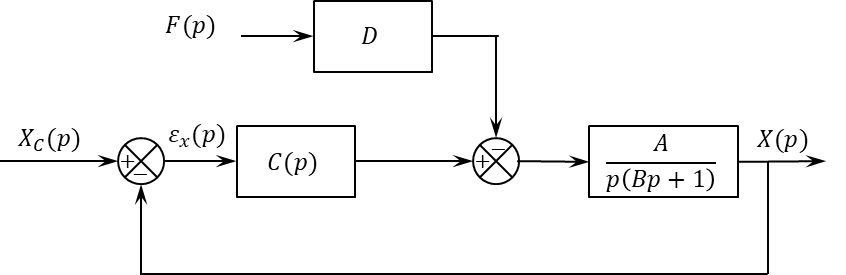
\includegraphics[width=\linewidth]{fig_08}
%\textit{}
\end{center}

Pour la suite du sujet on gardera les constantes $A$, $B$ et $D$, avec $A=\SI{6700}{m/V}$, $B=\SI{0,01}{s}$ et $D=\SI{6}{V/N}$.

\fi
\subsection*{Correction proportionnelle}

On suppose que $C(p)=K_c$. 


\question{Exprimer $\varepsilon_x$ en fonction des deux entrées $F_p$ et $X_c$ et des constantes $A$, $B$, $D$ et $K_c$.}
\ifprof
\begin{corrige}~\\
On a $\varepsilon_x(p)=X_C(p)-X(p)$ 
$ =X_C(p)-\left(\left(C(p)\varepsilon_x(p)-F(p)D \right)\dfrac{A}{p\left(Bp+1 \right)}  \right) $

$\Leftrightarrow \varepsilon_x(p) \left(1+ \dfrac{AC(p)}{p\left(Bp+1 \right)}\right)=X_C(p)+\dfrac{AF(p)D }{p\left(Bp+1 \right)}   $

$\Leftrightarrow \varepsilon_x(p) \left( \dfrac{p\left(Bp+1 \right)+AC(p)}{p\left(Bp+1 \right)}\right)=X_C(p)+\dfrac{AF(p)D }{p\left(Bp+1 \right)}   $
$\Leftrightarrow \varepsilon_x(p) =\dfrac{p\left(Bp+1 \right)}{p\left(Bp+1 \right)+AC(p)}X_C(p)+\dfrac{AF(p)D }{p\left(Bp+1 \right)+AC(p)}  $

$\Leftrightarrow \varepsilon_x(p) =\dfrac{p\left(Bp+1 \right)}{p\left(Bp+1 \right)+AK_C}X_C(p)+\dfrac{AD }{p\left(Bp+1 \right)+AK_C} F(p) $
\end{corrige}
\else
\fi



\question{Déterminer l'écart de position $\varepsilon_x$ en réponse à deux échelons d'intensité $F_0$ pour la force du patient et $X_0$ pour le déplacement. Conclure quant au respect du cahier des charges.}
\ifprof
\begin{corrige}~\\

On a : 
$\varepsilon_x = \lim_{p\to 0} p\varepsilon_x(p) = \lim_{p\to 0} p\left(\dfrac{p\left(Bp+1 \right)}{p\left(Bp+1 \right)+AK_C}\dfrac{X_0}{p}+\dfrac{AD }{p\left(Bp+1 \right)+AK_C} \dfrac{F_p}{p}\right) $

$= \lim_{p\to 0} \dfrac{p\left(Bp+1 \right)}{p\left(Bp+1 \right)+AK_C}{X_0}+\dfrac{AD }{p\left(Bp+1 \right)+AK_C} {F_p} $

$= \dfrac{D }{K_C} {F_p} $

L'écart en position n'est donc pas nul.
\end{corrige}
\else
\fi

\question{Tracer le diagramme de Bode de la FTBO du système pour $K_C=1$ et donner les marges. Le cahier des charges est-il vérifié ?}
\ifprof
\begin{corrige}~\\
On a $\text{FTBO}(p)=\dfrac{A}{p\left(Bp+1\right)}$.
\begin{center}
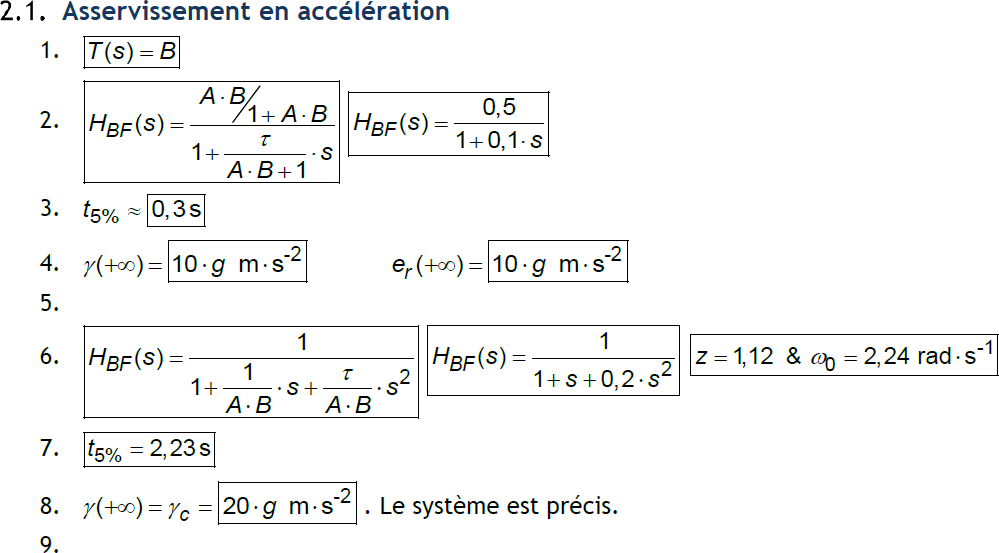
\includegraphics[width=\linewidth]{cor_02}
%\textit{}
\end{center}

La marge de phase n'est pas respectée. 

\end{corrige}
\else
\fi

\subsection*{Correction proportionnelle intégrale}
On suppose maintenant que $C(p)=K_i\left(1+\dfrac{1}{T_ip}\right)$

\question{Exprimer $\varepsilon_x$ en fonction des deux entrées $F_p$ et $X_c$ et des constantes $A$, $B$, $D$ et $K_i$.}
\ifprof
\begin{corrige}~\\


$\varepsilon_x(p) =\dfrac{p\left(Bp+1 \right)}{p\left(Bp+1 \right)+AK_i\left(1+\dfrac{1}{T_ip}\right)}X_C(p)+\dfrac{AD }{p\left(Bp+1 \right)+AK_i\left(1+\dfrac{1}{T_ip}\right)} F(p) $

\end{corrige}
\else
\fi

\question{Déterminer l'écart de position $\varepsilon_x$ en réponse à deux échelons d'intensité $F_0$ pour la force du patient et $X_0$ pour le déplacement. Conclure quant au respect du cahier des charges.}
\ifprof
\begin{corrige}~\\

$\varepsilon_x =\lim_{p\to 0} p\left(\dfrac{p\left(Bp+1 \right)}{p\left(Bp+1 \right)+AK_i\left(1+\dfrac{1}{T_ip}\right)}\dfrac{X_0}{p}+\dfrac{AD }{p\left(Bp+1 \right)+AK_i\left(1+\dfrac{1}{T_ip}\right)} \dfrac{F_0}{p}\right) $

$=\lim_{p\to 0} \dfrac{pT_ip\left(Bp+1 \right)}{pT_ip\left(Bp+1 \right)+AK_i\left(T_ip+1\right)}X_0+\dfrac{ADT_ip }{T_ipp\left(Bp+1 \right)+AK_i\left(T_ip+1\right)} F_0  = 0$.


\end{corrige}
\else
\fi


\question{Déterminer la fonction de transfert en boucle ouverte du système $\text{FTBO}(p)=\dfrac{X(p)}{\varepsilon_x(p)}$ en supposant que $F_p=0$.}
\ifprof
\begin{corrige}~\\
$\text{FTBO}(p)= \dfrac{A}{p\left(Bp+1\right)}K_i\left(1+\dfrac{1}{T_ip}\right)= \dfrac{A}{p\left(Bp+1\right)}K_i\dfrac{1+T_ip}{T_ip}$.


\end{corrige}
\else
\fi

\question{Déterminer la valeur $T_i$ permettant d'assurer la marge de phase pour la pulsation au gain unité souhaitée (pulsation pour laquelle le gain en décibel est nul).}
\ifprof
\begin{corrige}~\\
On souhaite que  pour $\omega=\SI{50}{rad.s^{-1}}$, $\varphi(\omega)=-135\degres $.

$\arg\left(\text{FTBO}(j\omega)\right) =\arg\left(\dfrac{A}{p\left(Bp+1\right)}K_i\dfrac{1+T_ip}{T_ip}\right)	$
$ =-180-\arg\left(\left(Bp+1\right)\right)  + \arg\left(1+T_ip\right)	$

$ =-180-\arctan B\omega + \arctan T_i \omega 	$
En $\omega=\SI{50}{rad.s^{-1}}$ on a alors 
$ -180-\arctan 0,5 + \arctan 50T_i =-135 \Leftrightarrow  \arctan 50T_i =-135+180+\arctan 0,5 =74$. D'où $T_i = \SI{0,05}{s}$.
\end{corrige}
\else
\fi


\question{Déterminer $K_i$ permettant d'assurer la pulsation au gain unité souhaitée.}


\ifprof
\begin{corrige}~\\
On souhaite que $|\text{FTBO}(j\omega)|=1$ pour $\omega=\SI{50}{rad.s^{-1}}$.

$|\text{FTBO}(j\omega)| =\left|\dfrac{A}{p\left(Bp+1\right)}K_i\dfrac{1+T_ip}{T_ip}\right|$
$=A K_i\dfrac{1}{\omega \sqrt{B^2\omega^2+1}}\dfrac{\sqrt{1+T_i^2\omega^2}}{T_i \omega }$
$=\dfrac{A K_i}{T_i \omega^2}\dfrac{\sqrt{1+T_i^2\omega^2}}{ \sqrt{B^2\omega^2+1}}$.

On a donc $K_i = \dfrac{T_i \omega^2\sqrt{B^2\omega^2+1}}{A\sqrt{1+T_i^2\omega^2}}=\SI{0,0077}{Vm^{-1}}$.

\end{corrige}
\else
\fi

On donne sur le document réponse la réponse temporelle du système à une entrée de type échelon unitaire sur le déplacement ($F_p=0$) ainsi que le diagramme de Bode de la FTBO.

\question{Conclure quant au respect du cahier des charges sur le reste des critères énoncés. Faire apparaître sur le document réponse les grandeurs mesurées.}
\ifprof
\begin{corrige}~\\
\begin{itemize}
\item Ecart de position : nul $\Rightarrow$ Exigence OK.
\item Marge de gain : infine $\Rightarrow$ Exigence OK.
\item Marge de phase : $\simeq 45\degres$ $\Rightarrow$ Exigence OK.
\end{itemize}

\begin{center}
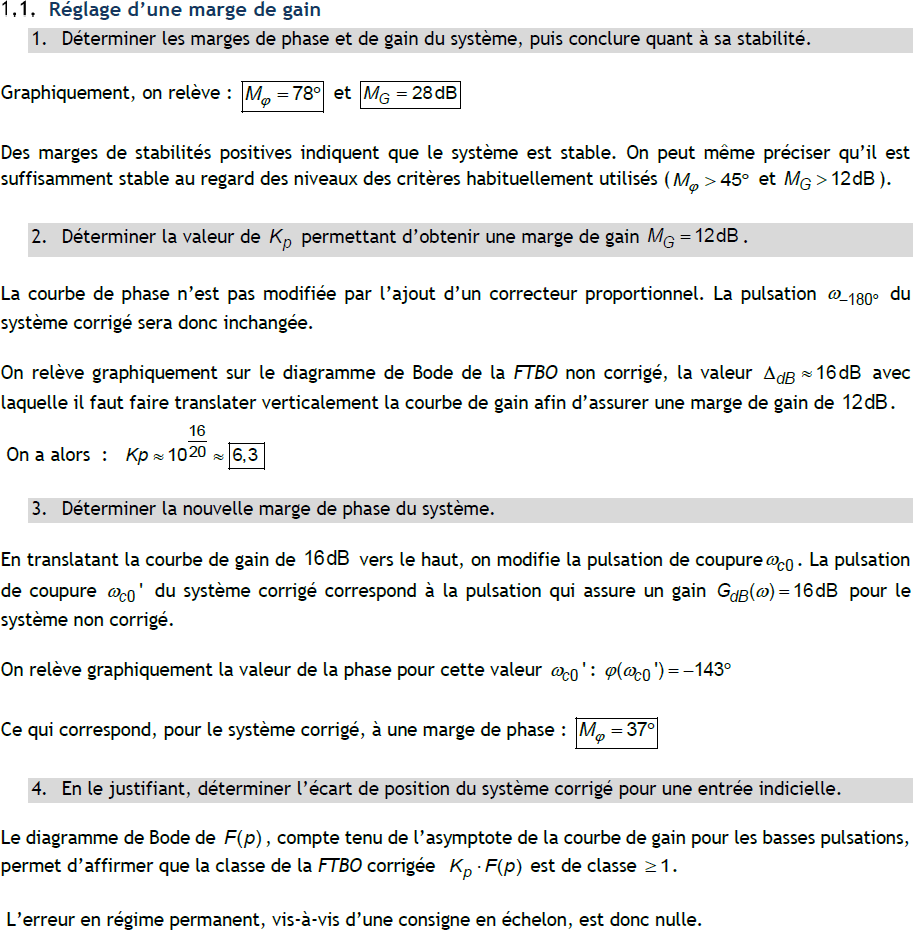
\includegraphics[width=\linewidth]{cor_03}
%\textit{}
\end{center}
 
\end{corrige}
\else
\fi


\ifprof
\else
\begin{center}
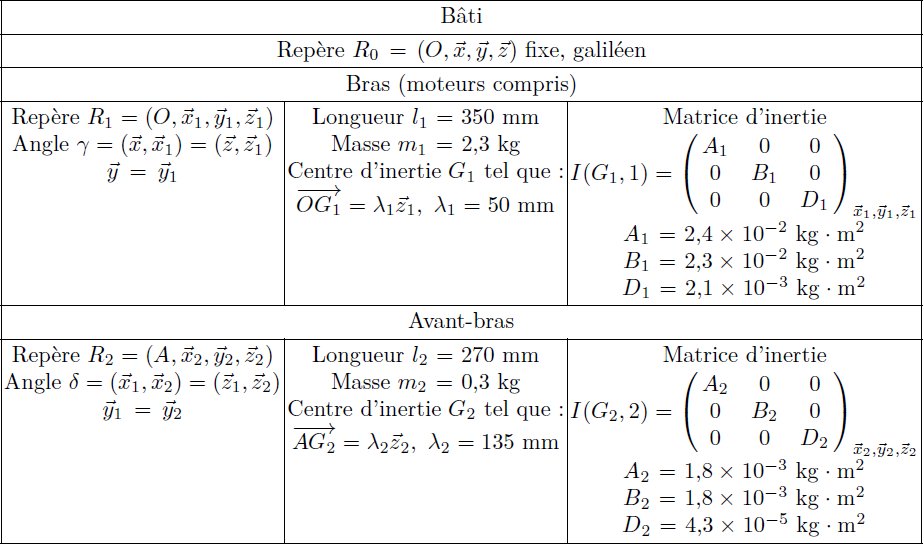
\includegraphics[width=\linewidth]{fig_06}
%\textit{}
\end{center}

\begin{center}
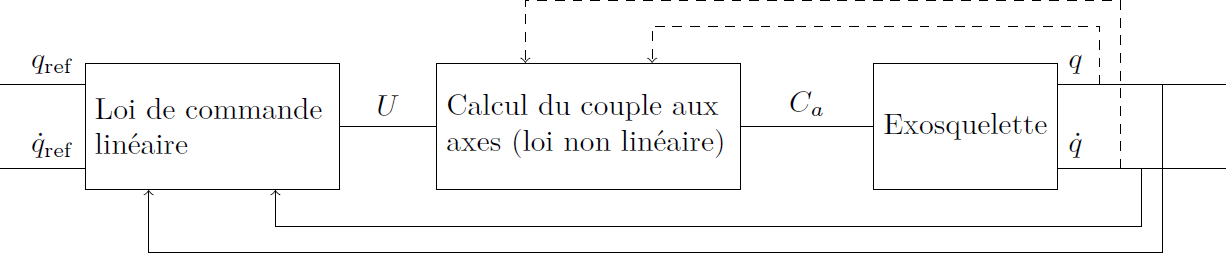
\includegraphics[width=\linewidth]{fig_07}
%\textit{}
\end{center}
\fi

\ifprof
\else
\end{multicols}
\fi



%
%\end{document}
%
%\question{}
%\ifprof
%\begin{corrige}~\\
%\end{corrige}
%\else
%\fi
%
%\begin{center}
%\includegraphics[width=\linewidth]{img_04}
%%\textit{}
%\end{center}
%
%
%\question{}
%\ifprof
%\begin{corrige}~\\
%\end{corrige}
%\else
%\fi
%
%\question{}
%\ifprof
%\begin{corrige}~\\
%\end{corrige}
%\else
%\fi
%
%\question{}
%\ifprof
%\begin{corrige}~\\
%\end{corrige}
%\else
%\fi
%
%\question{}
%\ifprof
%\begin{corrige}~\\
%\end{corrige}
%\else
%\fi
%
%\question{}
%\ifprof
%\begin{corrige}~\\
%\end{corrige}
%\else
%\fi
%
%\question{}
%\ifprof
%\begin{corrige}~\\
%\end{corrige}
%\else
%\fi
%\begin{center}
%%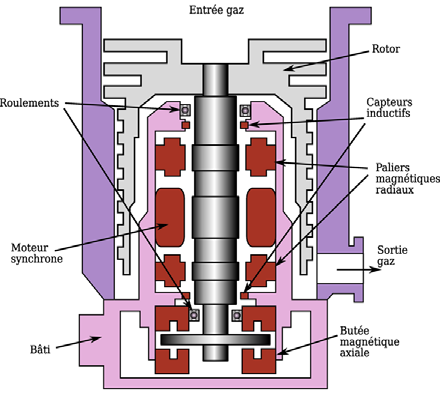
\includegraphics[width=\linewidth]{fig_05}
%\end{center}
